\documentclass[tikz,border=6pt]{standalone}

\usepackage{amsmath}
\usepackage{sansmath}
\usepackage{xcolor}
\usetikzlibrary{arrows.meta}

\definecolor{coltreat}{HTML}{0066CC}
\definecolor{colout}{HTML}{D62828}
\definecolor{collatent}{HTML}{A6A6A6}
\definecolor{filllatent}{HTML}{F2F2F2}
\definecolor{colvalid}{HTML}{2E8B57}
\definecolor{colinvalid}{HTML}{C76E00}

\begin{document}
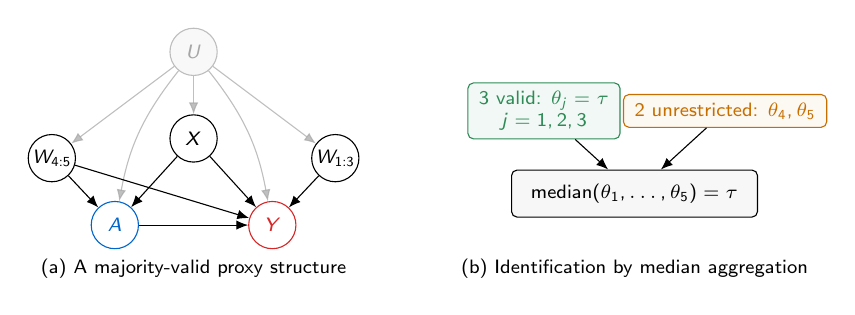
\begin{tikzpicture}[
  x=1cm,
  y=1cm,
  >={Latex[width=1.2mm,length=1.5mm]},
  font=\sffamily\sansmath\scriptsize,
  varnode/.style={draw,circle,inner sep=0mm,minimum size=6mm,
    font=\sffamily\sansmath\scriptsize},
  observed/.style={varnode,draw=black,text=black,fill=white},
  latent/.style={varnode,draw=collatent,draw opacity=0.72,text=collatent,
    fill=filllatent,fill opacity=0.55,text opacity=1},
  treatment/.style={varnode,draw=coltreat,text=coltreat,fill=white},
  outcome/.style={varnode,draw=colout,text=colout,fill=white},
  observed edge/.style={->,draw=black,line width=0.4pt},
  latent edge/.style={->,draw=collatent,opacity=0.72,line width=0.4pt},
  valid value/.style={draw=colvalid,rounded corners=2pt,text=colvalid,
    fill=colvalid!6,inner xsep=4pt,inner ysep=3pt},
  other value/.style={draw=colinvalid,rounded corners=2pt,text=colinvalid,
    fill=colinvalid!5,inner xsep=4pt,inner ysep=3pt},
  median/.style={draw=black,rounded corners=2pt,fill=black!3,
    inner xsep=7pt,inner ysep=5pt}
]

% Panel (a): grouped majority-valid proxy structure.
\begin{scope}[xshift=0cm]
  \node[latent] (U) at (0,1.55) {$U$};
  \node[observed] (X) at (0,0.45) {$X$};
  \node[treatment] (A) at (-1.00,-0.65) {$A$};
  \node[outcome] (Y) at (1.00,-0.65) {$Y$};
  \node[observed] (W45) at (-1.80,0.20) {$W_{4:5}$};
  \node[observed] (W13) at (1.80,0.20) {$W_{1:3}$};

  \draw[latent edge] (U) -- (X);
  \draw[latent edge] (U) -- (W13);
  \draw[latent edge] (U) -- (W45);
  \draw[latent edge] (U) to[bend right=14] (A);
  \draw[latent edge] (U) to[bend left=14] (Y);

  \draw[observed edge] (X) -- (A);
  \draw[observed edge] (X) -- (Y);
  \draw[observed edge] (A) -- (Y);
  \draw[observed edge] (W13) -- (Y);
  \draw[observed edge] (W45) -- (A);
  \draw[observed edge] (W45) -- (Y);

  \node[font=\sffamily\sansmath\scriptsize] at (0,-1.20)
    {(a) A majority-valid proxy structure};
\end{scope}

% Panel (b): compact median aggregation.
\begin{scope}[xshift=5.60cm]
  \node[valid value,align=center] (Tvalid) at (-1.15,0.80)
    {3 valid: $\theta_j=\tau$\\$j=1,2,3$};
  \node[other value,align=center] (Tother) at (1.15,0.80)
    {2 unrestricted: $\theta_4,\theta_5$};
  \node[median] (M) at (0,-0.25)
    {$\operatorname{median}(\theta_1,\ldots,\theta_5)=\tau$};

  \draw[observed edge] (Tvalid) -- (M);
  \draw[observed edge] (Tother) -- (M);

  \node[font=\sffamily\sansmath\scriptsize] at (0,-1.20)
    {(b) Identification by median aggregation};
\end{scope}

\end{tikzpicture}
\end{document}
